\section{Introduction}
\bigskip
\subsection{Initial situation}
\bigskip
The openETCS project has the goal to develop a semi-formal OBU model followed by a strictly formal one realizing functionalities of the UNISIG SRS-SUBSET-026, baseline 3, required for running on the ETCS level 2 of the Utrecht-Amsterdam track. The purpose of this formal model is to increase and spread consistent understanding of the subset, where it can be used as an artifact for testing, analyzing, verification and validation and also for further development pur-poses by industrial actors. This shall be achieved within a framework that is based on an open source concept. The ETCS On Board Unit EVC software model depicted in Figure 1 will be the focus of the software assessment according to the EN 50128:2011.

\begin{figure}
\label{toplevelarchitecture} 
\centering
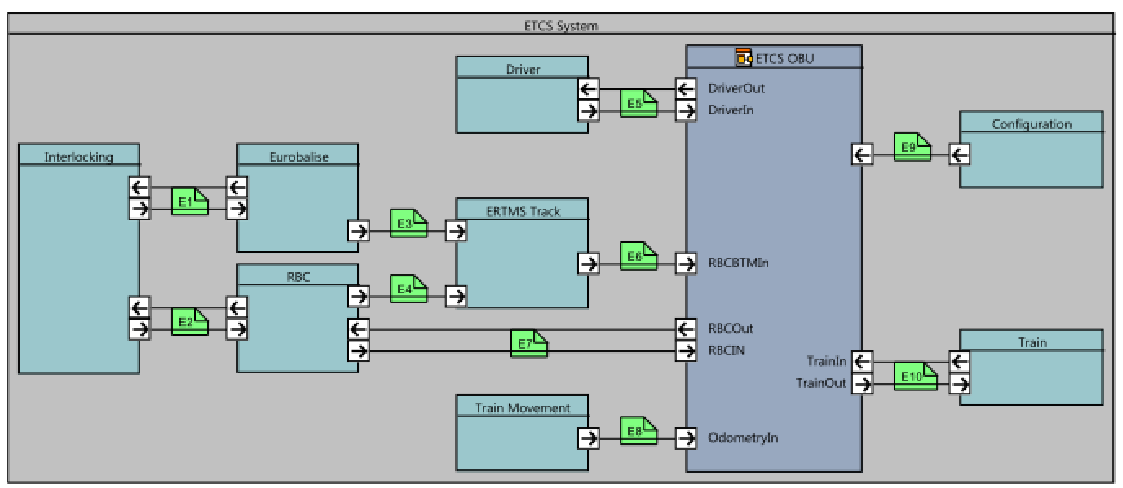
\includegraphics[width=14.552cm,height=6.35cm]{../images/toplevelarchitecture.pdf}
\captionof{figure}{Top level architecture view of the ETCS OBU}
\end{figure}



\bigskip

\subsection{Scope of the assessment}
\bigskip
The scope of the assessment will be the openETCS OBU Software. As it is stated in the Assessment Plan this will cover three main categories:

%\liststyleLiv
\begin{itemize}
\item Project and Software Quality assurance 
\item Verification \& Validation and 
\item Safety 
\end{itemize}

\bigskip

\subsection{Contents of the assessment and issues of concern}
\bigskip
The purpose of this assessment is to answer the following questions relating to software development:

\begin{enumerate}
	\item What measures have been taken to satisfy EN 50128?
	\item Are the measures taken for satisfying EN 50128 SIL 4 sufficient?
	\item Is the agile development practiced in the openETCS project complying with requirements of the EN 50128:2011?
\end{enumerate}
\bigskip

\subsection{Assessment conditions and exceptions}
\bigskip

The ETCS OBU software model has been developed with the closed source SCADE Suite of the company ESTEREL Technology and the code generated is SIL4 certified. Hence only the deliverables of the openETCS software development will have the scope of the
assessment. Also the SoftwareHardware integration is out of the scope of the assessment

\subsection{Documents for the software life cycle and software creation}
\bigskip
The following documents, which describe the software creation process, have been made available to the assessors.


\bigskip

{fixme}% Here i would prefer to add a LaTex Table with only the three columns: 
%1. Documentation (based on EN 50128)
%2. Mapped openETCS (bases on 2.3a Hardis document)
%3. Available openETCS derliverables

\begin{figure}
\label{documentmapping} 
\centering
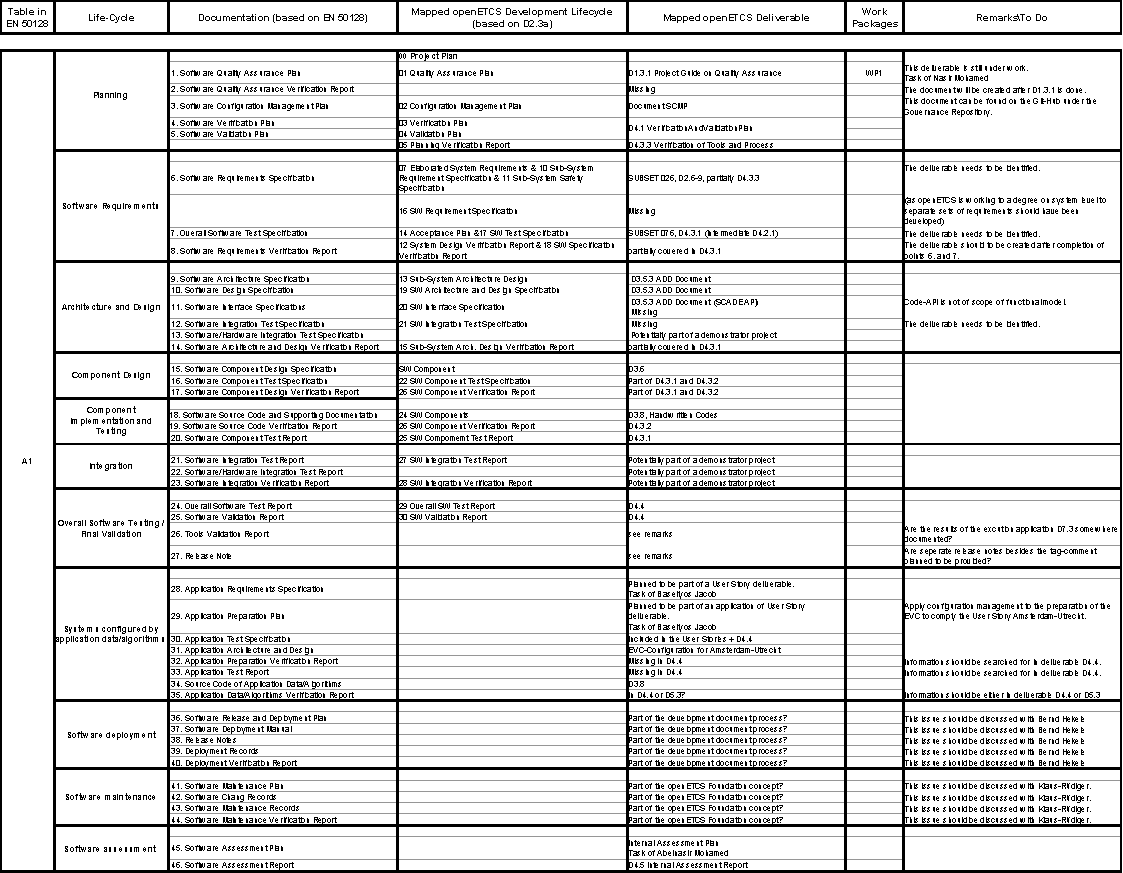
\includegraphics[width=21.001cm,height=16.341cm,angle=-90]{../images/documentmapping.pdf}
\captionof{figure}{Mapping of openETCS Documents to the CENELEC Lifecycle}
\end{figure}



